\documentclass{beamer}
\usepackage[utf8]{inputenc}
\usepackage[T1]{fontenc}
% \usepackage{amscd, amsfonts, amsmath, amssymb, amstext, amsthm, caption, epsfig, fancyhdr, float, graphicx, latexsym, mathtools, multicol, multirow, algorithm, chngcntr}
\usepackage[english]{babel}
\usepackage{booktabs}

\usepackage{amsmath,amssymb}
\usepackage{graphicx}
\usepackage{caption}
\usepackage{subfig}
\usepackage{xspace}
\usepackage{fourier}

\usepackage{tikz}
\usetikzlibrary{shapes,arrows}
\usepackage{tkz-graph}
\usetikzlibrary{automata,arrows,positioning,calc}
\usetikzlibrary{positioning}
\usetikzlibrary{fit}
\usetikzlibrary{backgrounds}
\usetikzlibrary{calc}
\usetikzlibrary{shapes}
\usetikzlibrary{mindmap}
\usetikzlibrary{decorations.text}
\usetikzlibrary{snakes}

% \theoremstyle{definition} % insert bellow all blocks you want in normal text
% \newtheorem{definition}{Definition}



% tikzmark command, for shading over items
\newcommand{\tikzmark}[1]{\tikz[overlay,remember picture] \node (#1) {};}
% Define block styles
\tikzstyle{decision} = [diamond, draw, fill=blue!20,
    text width=4.5em, text badly centered, node distance=3cm, inner sep=0pt]
\tikzstyle{block} = [rectangle, draw, fill=blue!20,
    text width=5em, text centered, rounded corners]
\tikzstyle{line} = [draw]
\tikzstyle{cloud} = [draw, ellipse,fill=red!20, node distance=3cm,
    minimum height=2em]

\usepackage[most]{tcolorbox}

\setbeamertemplate{blocks}[rounded][shadow=true] % use rounded blocks with standard beamer shadow


% Distributions.
\newcommand*{\UnifDist}{\mathsf{Unif}}
\newcommand*{\ExpDist}{\mathsf{Exp}}
\newcommand*{\DepExpDist}{\mathsf{DepExp}}
\newcommand*{\GammaDist}{\mathsf{Gamma}}
\newcommand*{\LognormalDist}{\mathsf{LogNorm}}
\newcommand*{\WeibullDist}{\mathsf{Weib}}
\newcommand*{\ParetoDist}{\mathsf{Par}}
\newcommand*{\NormalDist}{\mathsf{Norm}}

\newcommand*{\GeometricDist}{\mathsf{Geom}}
\newcommand*{\NegBinomialDist}{\mathsf{NegBin}}
\newcommand*{\PoissonDist}{\mathsf{Poisson}}
\newcommand*{\BivariatePoissonDist}{\mathsf{BPoisson}}
\newcommand*{\CyclicalPoissonDist}{\mathsf{CPoisson}}

\newcommand*{\iid}{\textbf{iid}\@\xspace}
\newcommand*{\pdf}{\textbf{pdf}\@\xspace}
\newcommand*{\cdf}{\textbf{cdf}\@\xspace}
\newcommand*{\pmf}{\textbf{pmf}\@\xspace}
\newcommand*{\abc}{{\textbf{abc}}\@\xspace}
\newcommand*{\smc}{\textbf{smc}\@\xspace}
\newcommand*{\mcmc}{\textbf{mcmc}\@\xspace}
\newcommand*{\ess}{\textbf{ess}\@\xspace}
\newcommand*{\mle}{\textbf{mle}\@\xspace}
\newcommand*{\bic}{\textbf{bic}\@\xspace}
\newcommand*{\kde}{\textbf{kde}\@\xspace}
\newcommand*{\glm}{\textbf{glm}\@\xspace}
\newcommand*{\xol}{\textbf{xol}\@\xspace}
\newcommand*{\cpu}{\textbf{cpu}\@\xspace}
\newcommand*{\gpu}{\textbf{gpu}\@\xspace}
\newcommand*{\arm}{\textbf{arm}\@\xspace}

\def \si {\sigma}
\def \la {\lambda}
\def \al {\alpha}
% \def\e*{\end{eqnarray*}}
\def \di{\displaystyle}

\def \E{\mathbb E}
\def \N{\mathbb N}
\def \Z{\mathbb Z}
\def \NZ{\mathbb{N}_0}
\def \I{\mathbb I}
\def \w{\widehat}
\def \P {\mathbb P}
\def \V{\mathbb V}


\newcommand{\CL}{\mathbb{C}}
\newcommand{\RL}{\mathbb{R}}
\newcommand{\nat}{{\mathbb N}}
\newcommand{\Laplace}{\mathscr{L}}
\newcommand{\e}{\mathrm{e}}
\newcommand{\ve}{\bm{\mathrm{e}}} % vector e

\renewcommand{\L}{\mathcal{L}} % e.g. L^2 loss.

\newcommand{\ih}{\mathrm{i}}
\newcommand{\oh}{{\mathrm{o}}}
\newcommand{\Oh}{{\mathcal{O}}}
\newcommand{\Exp}{\mathbb{E}}

\newcommand{\Norm}{\mathcal{N}}
\newcommand{\LN}{\mathcal{LN}}
\newcommand{\SLN}{\mathcal{SLN}}

\renewcommand{\Pr}{\mathbb{P}}
\newcommand{\Ind}{\mathbb I}
\newcommand\bfsigma{\bm{\sigma}}
\newcommand\bfSigma{\bm{\Sigma}}
\newcommand\bfLambda{\bm{\Lambda}}
\newcommand{\stimes}{{\times}}
\def \limsup{\underset{n\rightarrow+\infty}{\overline{\lim}}}
\def \liminf{\underset{n\rightarrow+\infty}{\underline{\lim}}}




% vertical separator macro
\newcommand{\vsep}{
  \column{0.0\textwidth}
    
\begin{tikzpicture}
      \draw[very thick,black!10] (0,0) -- (0,7.3);
    \end{tikzpicture}
}
\newcommand\blfootnote[1]{%
  \begingroup
  \renewcommand\thefootnote{}\footnote{#1}%
  \addtocounter{footnote}{-1}%
  \endgroup
}

% More space between lines in align
% \setlength{\mathindent}{0pt}

% Beamer theme
\usetheme{ZMBZFMK}
\usefonttheme[onlysmall]{structurebold}
\mode<presentation>
\setbeamercovered{transparent=10}

% align spacing
\setlength{\jot}{0pt}

\setbeamertemplate{navigation symbols}{}%remove navigation symbols

\title[BLOCKASTICS]{Stochastic models for blockchain analysis}
\author{Pierre-O. Goffard}
\institute[UNISTRA]{Université de Strasbourg\\
 \texttt{goffard@unistra.fr}
}
\date{\today}
% \titlegraphic{\includegraphics[width=2.5cm]{../../Figures/bfs_logo.png}} 

\begin{document}
\begin{frame}
  \titlepage
\end{frame}
\begin{frame}
  \tableofcontents
\end{frame}

\section{Introduction}
\begin{frame}{Blockchain}
A decentralized data ledger made of blocks maintained by achieving consensus in a P2P network.
\begin{columns}
\begin{column}{0.5\textwidth}
% \small

\begin{itemize}
  \item Decentralized
  \item Public/private
  \item Permissionned/permissionless
  \item Immutable
  \item Incentive compatible
\end{itemize}
\end{column}
\begin{column}{0.5\textwidth}
\begin{center}
\begin{tikzpicture}[-, >=stealth', auto, semithick, node distance=01cm]
\tikzstyle{every edge}=[snake=expanding waves,segment length=1mm,segment angle=10, draw]

\tikzstyle{full node}=[circle, fill=tublue,draw=tublue,thick,text=black,scale=0.8]
\tikzstyle{light node}=[circle, fill=white,draw=tublue,thick,text=black,scale=0.8]
\node[full node]    (1)                     {};
\node[full node]    (2)[above right of=1]         {};
\node[full node]    (3)[above left of=1]         {};
\node[full node]    (4)[below of=1]         {};
\node[full node]    (5)[right of=4]         {};
\node[full node]    (6)[below of=4]         {};
\node[light node]    (7)[left of=1]         {};
\node[light node]    (8)[right of=2]         {};
\node[light node]    (9)[left of=4]         {};
\node[light node]    (10)[above right of=5]         {};
\node[light node]    (11)[ right of=5]         {};
\node[light node]    (12)[ below right of=5]         {};
% \node[light node]    (4)[above of=2]         {};
\path

(1) edge node{} (2)
    edge node{} (3)
    edge node{} (7)
    ;
\path
(5) edge node{} (10)
    edge node{} (11)
    edge node{} (12)
    ;
    \path
(4) edge node{} (5)
    edge node{} (1)
    edge node{} (9)
    edge node{} (6)
    ;
    \path
(2) edge node{} (8)   
    ;
\end{tikzpicture}
\end{center}
\end{column}
\end{columns}

\vspace{0.2cm}
\begin{tcolorbox}[enhanced,drop shadow, title=Focus of the talk]
Public and permissionless blockchain equipped with the Proof-of-Work protocol.
\end{tcolorbox}
\end{frame}

\begin{frame}{Consensus protocols}
The mechanism to make all the nodes agree on a common data history.\\
\vspace{0.3cm}
The three dimensions of blockchain systems analysis
\begin{enumerate}
  \item Efficiency
  \begin{itemize}
    \item Throughputs
    \item Transaction confirmation time
  \end{itemize}
  \item Decentralization
  \begin{itemize}
    \item Fair distribution of the accounting right
  \end{itemize}
  \item Security 
  \begin{itemize}
    \item Resistance to attacks
  \end{itemize}
\end{enumerate}
\footnotesize
\begin{thebibliography}{1}
\bibitem{Fu2020}
X.~Fu, H.~Wang, and P.~Shi, ``A survey of blockchain consensus algorithms:
  mechanism, design and applications,'' {\em Science China Information
  Sciences}, vol.~64, nov 2020.
\end{thebibliography}
\end{frame}
\begin{frame}{Applications of blockchain: Cryptocurrency}
\begin{columns}
\begin{column}{0.5\textwidth}
   
{\footnotesize
\begin{thebibliography}{1}
\bibitem{Na08}
S.~Nakamoto, ``Bitcoin: A peer-to-peer electronic cash system.'' Available at
  \href{https://bitcoin.org/bitcoin.pdf}{https://bitcoin.org/bitcoin.pdf},
  2008.
\end{thebibliography}  
}
\end{column}
\begin{column}{0.5\textwidth}  %%<--- here
    \begin{center}
     \includegraphics[width=0.5\textwidth]{../../Figures/bitcoin-6284869_1920.png}
     \end{center}
\end{column}
\end{columns}

\begin{itemize}
  \item Transaction anonymity
  \item Banking and reliable currency in certain regions of the world
  \item Money Transfer worldwide (at low fare)
  \item No need for a thrusted third party
\end{itemize}
\end{frame}
\begin{frame}{Decentralized finance}
DEFI creates new financial architecture
\begin{columns}
\begin{column}{0.5\textwidth}
\begin{itemize}
\item[+] Non custodial
\item[+] Anonymous
\item[+] Permisionless
\item[+] openly auditable
\end{itemize}
\end{column}
\begin{column}{0.5\textwidth} 
\begin{itemize}
\item[-] Unregulated
\item[-] Tax evasion
\item[-] Fraud
\item[-] Money laundering
\end{itemize} 
\end{column}
\end{columns}
\vspace{0.5cm}
Extends the Bitcoin promises to more complex financial operations
\begin{itemize}
  \item Collateralized lending
  \item Decentralized Exchange Platform
  \item Tokenized assets
  \item Fundraising vehicle (ICO, STO, ...)
\end{itemize}
\vspace{0.3cm}
\scriptsize
\begin{thebibliography}{1}

\bibitem{werner2021sok}
S.~M. Werner, D.~Perez, L.~Gudgeon, A.~Klages-Mundt, D.~Harz, and W.~J.
  Knottenbelt, ``Sok: Decentralized finance (defi),'' 2021.

\end{thebibliography}

\end{frame}
\begin{frame}{What's inside a block?}
A block consists of 
\begin{itemize}
\item a header 
\item a list of "transactions" that represents the information recorded through the blockchain. 
\end{itemize}
The header usually includes 
\begin{itemize}
\item the date and time of creation of the block, 
\item the block height which is the index inside the blockchain, 
\item the hash of the block 
\item the hash of the previous block. 
\end{itemize}
\begin{tcolorbox}[enhanced,drop shadow, title=Question]
What is the hash of a block?
\end{tcolorbox}
\end{frame}
\begin{frame}{Cryptographic Hash function}
\small
A function that maps data of arbitratry size (message) to a bit array of fixed size (hash value)
$$
h:\{0,1\}^\ast\mapsto \{0,1\}^d. 
$$
A good hash function is
\begin{itemize}
\item deterministic
\item quick to compute
\item One way
\begin{itemize}
  \scriptsize
\item[$\hookrightarrow$] For a given hash value $\overline{h}$ it is hard to find a message $m$ such that 
$$
h(m) = \overline{h}
$$
\end{itemize}
\item Colision resistant 
\begin{itemize}
\item[$\hookrightarrow$] Impossible to find $m_1$ and $m_2$ such that 
$$
h(m_1) = h(m_2)
$$
\end{itemize}
\item Chaotic
$$m_1\approx m_2\Rightarrow  h(m_1) \neq h(m_2)$$
\end{itemize}
\end{frame}
\begin{frame}{SHA-256}
The SHA-256 function which converts any message into a hash value of $256$ bits.
\begin{tcolorbox}[enhanced,drop shadow, title=Example]
The hexadecimal digest of the message
$$
\texttt{Is DeFi the future?}
$$
is 
\footnotesize
$$
\texttt{50f3257a3d22a56247a8978fd2505e8cdd64e1cb06e52c941d09e234722dc275}
$$
\end{tcolorbox}
\end{frame}
\begin{frame}{Mining a block}
\begin{figure}[!ht]
    \includegraphics[width = \textwidth]{../../Figures/block_not_mined.png}
    \captionsetup{width=0.8\textwidth}
    \centering
    \caption{A block that has not been mined yet.}
    \label{fig:block_not_mined}
\end{figure}
\end{frame}
\begin{frame}{Mining a block}
The maximum value for a 256 bits number is
$$
T_\text{max} = 2^{256}-1 \approx 1.16e^{77}.
$$
Mining consists in drawing at random a nonce 
$$
\text{Nonce} \sim \text{Unif}(\{0,\ldots, 2^{32}-1\}),
$$
until 
$$
h(\text{Nonce}|\text{Block info})<T,
$$
where $T$ is referred to as the target.
\begin{tcolorbox}[enhanced,drop shadow, title=Difficulty of the cryptopuzzle]
$$
D = \frac{T_{\max}}{T}.
$$
\end{tcolorbox}

\end{frame}
\begin{frame}{Mining a block}
If we set the difficulty to $D = 2^4$ then the hexadecimal digest must start with at least $1$ leading $0$
\begin{figure}[!ht]
    \includegraphics[width = \textwidth]{../../Figures/block_mined.png}
    \captionsetup{width=0.8\textwidth}
    \centering
    \caption{A mined block with a hash value having on leading zero.}
    \label{fig:block_mined}
\end{figure}
The number of trial is geometrically distributed
\begin{itemize}
\item Exponential inter-block times
\item Lenght of the blockchain = Poisson process
\end{itemize}
\end{frame}
\begin{frame}{Bitcoin protocol}
\begin{itemize}
  \item One block every 10 minutes on average
  \item Depends on the hashrate of the network
  \item Difficulty adjustment every 2,016 blocks ($\approx$ two weeks)
  \item Reward halving every 210,000 blocks
\end{itemize}
Check out \url{https://www.bitcoinblockhalf.com/}

\end{frame}
\section{Double spending attack}
\begin{frame}{Double spending attack}
\scriptsize
\begin{enumerate}
\item Mary transfers 10 BTCs to John
\item The transaction is recorded in the public branch of the blockchain and John ships the good.
\item Mary transfers to herself the exact same BTCs
\item The malicious transaction is recorded into a private branch of the blockchain
\begin{itemize}
  \scriptsize
\item Mary has friends among the miners to help her out
\item The two chains are copycat up to the one transaction
\end{itemize}
\end{enumerate}
\begin{tcolorbox}[enhanced,drop shadow, title=Fact (Bitcoin has only one rule)]
The longest chain is to be trusted
\end{tcolorbox}
\end{frame}
\begin{frame}{Double spending in practice}
\scriptsize
Vendor are advised to wait for $\alpha\in\mathbb{N}$ of confirmations so that the honest chain is ahead of the dishonest one.
\begin{center}
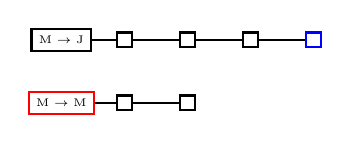
\begin{tikzpicture}[-, >=stealth', auto, semithick, node distance=1cm]
% \tikzstyle{block} = [rectangle, draw, fill=blue!20,
%     text width=5em, text centered, rounded corners]
\tikzstyle{block}=[rectangle, fill=black,draw=black,thick,text=black,scale=0.6]
\tikzstyle{block}=[rectangle, fill=white,draw=black,thick,text=black,scale=0.8]
\tikzstyle{confirmed block}=[rectangle, fill=white,draw=blue,thick,text=black,scale=0.8]
\tikzstyle{bad block}=[rectangle, fill=white,draw=red,thick,text=black,scale=0.8]
\node[block]    (1)                     {\tiny $\text{M}\rightarrow \text{J}$};
\node[block]    (2)[right of=1]                     {};
\node[block]    (3)[right of=2]                     {};
\node[block]    (4)[right of=3]                     {};
\node[confirmed block]    (5)[right of=4]                     {};

\node[bad block]    (6)[below of=1]         {\tiny $\text{M}\rightarrow \text{M}$};
\node[block]    (7)[right of=6]         {};
\node[block]    (8)[right of=7]         {};
\path
(1) edge[ left]     node{}     (2)
(2) edge[ left]     node{}     (3)
(3) edge[ left]     node{}     (4)
(4) edge[ left]     node{}     (5)
(6) edge[ left]     node{}     (7)
(7) edge[ left]     node{}     (8);

\end{tikzpicture}
\end{center}
In the example, vendor awaits $\alpha = 4$ confirmations, the honest chain is ahead of the dishonest one by $z = 2$ blocks.
\begin{tcolorbox}[enhanced,drop shadow, title=Fact (PoW is resistant to double spending)]
\begin{itemize}
\item Attacker does not own the majority of computing power 
\item Suitable $\alpha$ 
\end{itemize}
Double spending is unlikely to succeed.
\end{tcolorbox}
\tiny
\begin{thebibliography}{1}
\bibitem{Na08}
S.~Nakamoto, ``Bitcoin: A peer-to-peer electronic cash system.'' Available at
  \href{https://bitcoin.org/bitcoin.pdf}{https://bitcoin.org/bitcoin.pdf},
  2008.
  
\end{thebibliography}

\end{frame}
\begin{frame}{Mathematical set up}
\footnotesize
Assume that
\begin{itemize}
\item $R_0=z\geq1$ (the honest chain is z blocks ahead)
\item at each time unit a block is created
\begin{itemize}
  \footnotesize
\item[$\hookrightarrow$] in the honest chain with probability $p$
\item[$\hookrightarrow$] in the dishonest chain with probability $q=1-p$
\end{itemize}
\end{itemize}
The process $(R_n)_{n\geq0}$ is a random walk on $\mathbb{Z}$ with
$$R_n=z+Y_1+\ldots+Y_n,$$
where $Y_1,\ldots,Y_n$ are the \textbf{i.i.d.} steps of the random walk. 

\end{frame}
\begin{frame}{Double spending rate of success}
\scriptsize
Double spending occurs at time
$$
\tau_z=\inf\{n\in \mathbb{N}\text{ ; }R_n=0\}.
$$
\begin{tikzpicture}
  %Origin and axis
  \coordinate (O) at (0,0);
  \draw[->] (-1,0) -- (9,0) coordinate[label = {below:$n$}] (xmax);
  \draw[->] (0,-0.5) -- (0,3) coordinate[label = {left:$Z_n$}] (ymax);
  %Lower linear boundary

 
  %Stochastic process trajectory
  
  \draw (0,0) node[tublue,left] {} node{};
  \draw[very thick,tublue,-] (0,1) -- (1,1) node[pos=0.5, above] {} ;
  \draw[very thick,dashed,tublue] (1,1) -- (1,1.5) node[pos=0.5, right] {};
  \draw[very thick,tublue,-] (1,1.5) -- (2,1.5) node[pos=0.5, above] {};
  \draw[very thick,dashed,tublue] (2,1.5) -- (2,2) node[pos=0.5, right] {};
  \draw[very thick,tublue,-] (2,2) -- (3,2) node[pos=0.5, above] {};
  \draw[very thick,dashed,tublue] (3,2) -- (3,1.5) node[pos=0.5, right] {};
  \draw[very thick,tublue,-] (3,1.5) -- (4,1.5)node[pos=0.5, above] {};
  \draw[very thick,dashed,tublue] (4,1.5) -- (4,1) node[pos=0.5, right] {};  
  \draw[very thick,tublue,-] (4,1) -- (5,1) node[pos=0.5, above] {};
  \draw[very thick,dashed,tublue] (5,1) -- (5,0.5) node[pos=0.5, right] {};  
  \draw[very thick,tublue,-] (5,0.5) -- (6,0.5) node[pos=0.5, above] {};
  \draw[very thick,dashed,tublue,-] (6,0.5) -- (6,1) node[pos=0.5, above] {};
   \draw[very thick,tublue,-] (6,1) -- (7,1) node[pos=0.5, above] {};
    \draw[very thick,dashed,tublue,-] (7,1) -- (7,0.5) node[pos=0.5, above] {};
     \draw[very thick,tublue,-] (7,0.5) -- (8,0.5) node[pos=0.5, above] {};
     \draw[very thick,dashed,tublue,-] (8,0.5) -- (8,0) node[pos=0.5, above] {};
  %Jump Times
  \draw (1,0) node[black,below] {$1$} node{ \color{black}$\bullet$};
  \draw (2,0) node[black,below] {$2$} node{ \color{black}$\bullet$};
  \draw (3,0) node[black,below] {$3$} node{ \color{black}$\bullet$};
  \draw (4,0) node[black,below] {$4$} node{ \color{black}$\bullet$};
  \draw (5,0) node[black,below] {$5$} node{ \color{black}$\bullet$};
  \draw (6,0) node[black,below] {$6$} node{ \color{black}$\bullet$};
  \draw (7,0) node[black,below] {$7$} node{ \color{black}$\bullet$};
  \draw (8,0) node[black,below] {$8$} node{ \color{black}$\bullet$};
  %Level of the counting process
   \draw (0,0) node[black,below left] {$0$} node{ \color{black}$\bullet$};
   \draw (0,0.5) node[black,left] {$1$} node{ \color{black}$\bullet$};
   \draw (0,1) node[black,left] {$z=2$} node{ \color{black}$\bullet$};
   \draw (0,1.5) node[black,left] {$3$} node{ \color{black}$\bullet$};
   \draw (0,2) node[black,left] {$4$} node{ \color{black}$\bullet$};
   \draw (0,2.5) node[black,left] {$5$} node{ \color{black}$\bullet$};

  % %Aggregated Capital gains
%  \draw (0,1.5) node[blue,below right] {$\mu_1$} node{ \color{blue}$-$};
%  \draw (0,2.25) node[blue,left] {$\mu_2$} node{ \color{blue}$-$};
%  \draw (0,3.75) node[blue,left] {$\mu_3$} node{ \color{blue}$-$};
  %Ruin time = First-crossing time time
%  \draw (5,0) node[black,above right] {$\tau_u$} node{ \color{black}$\times$};
%  \draw[dotted,black] (0,3.28) -- (5,3.28);
%  \draw[dotted,black] (5,0) -- (5,3.28);
\end{tikzpicture}
\begin{tcolorbox}[enhanced,drop shadow, title=Double spending theorem]
If $p>q$ then the double-spending probability is given by
$$
\phi(z) = \mathbb{P}(\tau_z<\infty)=\left(\frac{q}{p}\right)^{z}.
$$
\end{tcolorbox}

\end{frame}
\begin{frame}{Refinements of the double spending problem}
\scriptsize
The number of blocks $M$ found by the attacker until the honest miners find $\alpha$ blocks is a negative binomial random variable with \pmf
$$
\mathbb{P}(M = m) = \binom{\alpha+m-1}{m}p^\alpha q^m,\text{ }m\geq0.
$$
The number of block that the honest chain is ahead of the dishonest one is given by 
$$
Z= (\alpha-M)_+.
$$
Applying the law of total probability yields the probability of successful double spending with
$$
\mathbb{P}(\text{Double Spending}) = \mathbb{P}(M\geq \alpha) + \sum_{m = 0}^{\alpha - 1}\binom{\alpha+m-1}{m}q^{\alpha} p^{m}.
$$ 
\tiny


\begin{thebibliography}{1}
  \bibitem{rosenfeld2014analysis}
M.~Rosenfeld, ``Analysis of hashrate-based double spending,'' {\em arXiv
  preprint arXiv:1402.2009}, 2014.
  \bibitem{GRUNSPAN2018}
C.~Grunspan and R.~Perez-Marco, ``Double spend race,'' {\em
  International Journal of Theoretical and Applied Finance}, vol.~21,
  p.~1850053, dec 2018.
\end{thebibliography}

\end{frame}
\begin{frame}{Refinements of the double spending problem}
\scriptsize
Let the length of honest and dishonest chain be driven by counting processes
\begin{itemize}
\item Honest chain $\Rightarrow$ $z+N_t\text{ , }t\geq0$, where $z\geq1$.
\item Malicious chain $\Rightarrow$ $M_t\text{ , }t\geq0$
\item Study the distribution of the first-\textit{rendez-vous} time
$$
\tau_z=\inf\{t\geq0\text{ , } M_t=z+N_t\}.
$$
\end{itemize}
If $N_t\sim\text{Pois}(\lambda t)$ and $M_t\sim\text{Pois}(\mu t)$ such that $\lambda>\mu$ then 
$$
\phi(z) = \left(\frac{\mu}{\lambda}\right)^z,\text{ }z\geq 0.
$$
\tiny
\begin{thebibliography}{1}

\bibitem{Goffard2019}
P.-O. Goffard, ``Fraud risk assessment within blockchain transactions,'' {\em
  Advances in Applied Probability}, vol.~51, pp.~443--467, jun 2019.
\newblock \url{https://hal.archives-ouvertes.fr/hal-01716687v2}.

\bibitem{Bowden2020}
R.~Bowden, H.~P. Keeler, A.~E. Krzesinski, and P.~G. Taylor, ``Modeling and
  analysis of block arrival times in the bitcoin blockchain,'' {\em Stochastic
  Models}, vol.~36, pp.~602--637, jul 2020.
\end{thebibliography}

\end{frame}

\section{Insurance risk theory}
\begin{frame}{Cramer-Lunberg model}
\begin{columns}
\begin{column}{0.5\textwidth}
\scriptsize
The financial reserves of an insurance company over time have the following dynamic
\begin{equation*}
R_t = z +ct - \sum_{i = 1}^{N_t}U_i\text{, }t\geq0,
\end{equation*}
where 
\begin{itemize}
  \item $z>0$ denotes the initial reserves
  \item $c$ is the premium rate
  \item $(N_t)_{t\geq0}$ is a counting process that models the claim arrival 
  \begin{itemize}
    \scriptsize
    \item[$\hookrightarrow$]  Poisson process with intensity $\lambda$
  \end{itemize}
  \item The $U_i$'s are the randomly sized compensations
  \begin{itemize}
    \scriptsize
    \item[$\hookrightarrow$] non-negative, \textbf{i.i.d.}
  \end{itemize}
\end{itemize}
\end{column}
\begin{column}{0.5\textwidth}
\begin{tikzpicture}
  %Origin and axis
  \coordinate (O) at (0,0);
  \draw[->] (-0.5,0) -- (5.5,0) coordinate[label = {below:\scriptsize$t$}] (xmax);
  \draw[->] (0,-0.5) -- (0,4) coordinate[label = {right:\scriptsize$R_t$}] (ymax);
   %Initial reserves
  \draw (0,2) node[black,left] {\scriptsize$z$} node{};
 % % %Length of the honest chain
  \draw[thick, tublue,-] (0,2) -- (2,3) node[pos=0.5, above] {};
  \draw[thick, dashed, tublue] (2,3) -- (2,1) node[pos=0.5, left] {\scriptsize\color{black}$U_1$};
  \draw[thick, tublue] (2,1) -- (3,1.5) node[pos=0.5, above] {};
  \draw[thick, dashed, tublue] (3,1.5) -- (3, 0.5) node[pos=0.5, left] {\scriptsize\color{black}$U_2$};
  \draw[thick, tublue] (3,0.5) -- (5, 1.5) node[pos=0.5, above] {};
   \draw[thick, dashed, tublue] (5,1.5) -- (5, -0.5) node[pos=0.5,above left] {\scriptsize\color{black}$U_3$};

  %Block finding Times 
  \draw (2,0) node[black,below] {\scriptsize$T_1$} node{ \color{black}$\bullet$};
  \draw (3,0) node[black,below] {\scriptsize$T_2$} node{ \color{black}$\bullet$};
  \draw (5,0) node[black,below left] {\scriptsize$\tau_z$} node{ \color{black}$\bullet$};
\end{tikzpicture}
\end{column}
\end{columns}

\end{frame}
\begin{frame}{Ruin probabilities}
\scriptsize
Define the ruin time as 
$$
\tau_z = \inf\{t\geq0\text{ ; }R_t <0\}
$$
and the ruin probabilities as 
$$
\psi(z,t) = \mathbb{P}(\tau_z < t)\text{ and }\psi(z) = \mathbb{P}(\tau_z < \infty)
$$
We look for $z$ such that 
$$
\mathbb{P}(\text{Ruin}) = \alpha\text{ (0.05)},
$$
given that 
$$
c=(1+\eta)\lambda\mathbb{E}(U),
$$
with 
$$\eta>0\text{ (net profit condition)}$$  
otherwise 
$$\psi(z)=1.$$

\tiny
\begin{thebibliography}{1}

\bibitem{Asmussen_2010}
S.~Asmussen and H.~Albrecher, {\em Ruin Probabilities}.
\newblock {WORLD} {SCIENTIFIC}, sep 2010.

\end{thebibliography}

\end{frame}

\begin{frame}{Ruin probability computation}
\scriptsize
Let 
$$
S_t = z - R_t,\text{ }t\geq0
$$
\begin{tcolorbox}[enhanced,drop shadow, title=Theorem (Wald exponential martingale)]
If $(S_t)_{t\geq0}$ is a L\'evy process or a random walk then
$$
\{\exp\left[\theta S_t-t\kappa(\theta)\right]\text{ , }t\geq0\},\text{ is a martingale,}
$$
where $\kappa(\theta)=\log\mathbb{E}\left(e^{\theta S_1}\right)$.
\end{tcolorbox}
\begin{tcolorbox}[enhanced,drop shadow, title=Theorem (Representation of the ruin probability)]

If $S_t\overset{\textbf{a.s.}}{\rightarrow} -\infty$, and there exists $\gamma>0$ such that $\{e^{\gamma S_t}\text{ , }t\geq0\}$ is a martingale then
$$
\mathbb{P}(\tau_z<\infty)=\frac{e^{-\gamma z}}{\mathbb{E}\left[e^{\gamma \xi(z)}|\tau_z<\infty\right]},
$$
where $\xi(z)=S_{\tau_z}-z\text{ denotes the deficit at ruin.}$
\end{tcolorbox}
\end{frame}
\begin{frame}{Sketch of Proof}
\scriptsize
\begin{itemize}
\item Because of the net profit condition $S_t = \sum_{i=1}^{N_t}U_i-ct\rightarrow -\infty$ as $t\rightarrow\infty$
\item $(S_t)_{t\geq0}$ is a Lévy process, let $\gamma$ be the (unique, positive) solution to
$$
\kappa(\theta) = 0\text{ (Cramer-Lundberg equation)}.
$$
\item  $(e^{\gamma S_t})_{t\geq0}$ is a Martingale then apply the Optional stopping theorem at $\tau_z$.

\end{itemize}
\end{frame}
\section{Link to double spending}
\begin{frame}{Double spending in Satoshi's framework}
\scriptsize
\begin{itemize}
\item The risk reserve process is $R_t=z+Y_1+\ldots+Y_t.$
\item The claim surplus process is $S_t=-(Y_1+\ldots+Y_t).$
\item $\kappa(\theta)=0$ is equivalent to
$$pe^{-\theta}+qe^{\theta}=1.$$
\begin{itemize}
\item[$\hookrightarrow$]\scriptsize $\gamma=\log(p/q).$
\end{itemize}
\item If $p>q$ then $S(t)\rightarrow - \infty$.
\item  $\xi(z)=S_{\tau_z}-z=0$ \textbf{a.s}.
\end{itemize}
Thus,
$$\mathbb{P}(\tau_z<\infty)=\left(\frac{q}{p}\right)^{z}.$$
\end{frame}

\begin{frame}{Double spending with Poisson processes}
\begin{columns}
\begin{column}{0.5\textwidth}
\scriptsize
\begin{itemize}
\item Suppose that
$$
N_t\sim\text{Pois}(\lambda t)\text{ and }M_t\sim\text{Pois}(\mu t)
$$
such that $\lambda>\mu$.
\item The risk reserve process is $R_t=z+N_t-M_t.$
\item The claim surplus process is $S_t=M_t-N_t.$
\end{itemize}
\begin{tcolorbox}[enhanced,drop shadow, title=Fact]
The difference of two Poisson processes is not a Poisson process, However it is L\'evy!
\end{tcolorbox}
\end{column}
\begin{column}{0.5\textwidth}
\begin{tikzpicture}
  %Origin and axis
  \coordinate (O) at (0,0);
  \draw[->] (-0.5,0) -- (5.5,0) coordinate[label = {above:\scriptsize$t$}] (xmax);
  \draw[->] (0,-0.5) -- (0,5) coordinate[label = {right:\scriptsize$n$}] (ymax);
 %Length of the honest chain
  \draw[thick,tublue,-] (0,3) -- (2,3) node[pos=0.5, above] {} ;
  \draw[thick,tublue] (2,3) -- (2,4) node[pos=0.5, above] {};
  \draw[thick,tublue] (2,4) -- (5.5,4) node[pos=0.5, right] {};
  % %Length of the Malicious chain
  \draw[very thick,dashed,red,-] (0,0) -- (0.75,0) node[pos=0.5, above] {} ;
  \draw[very thick,dashed,red] (0.75,0) -- (0.75,1) node[pos=0.5, right] {};
  \draw[very thick,dashed,red] (0.75,1) -- (1.25,1) node[pos=0.5, above] {};
  \draw[very thick,dashed,red] (1.25,1) -- (1.25,2) node[pos=0.5, right] {};
  \draw[very thick,dashed,red] (1.25,2) -- (2.5,2) node[pos=0.5, above] {};
  \draw[very thick,dashed,red] (2.5,2) -- (2.5,3) node[pos=0.5, right] {};
  \draw[very thick,dashed,red] (2.5,3) -- (5,3) node[pos=0.5, right] {};
  \draw[very thick,dashed,red] (5,3) -- (5,4) node[pos=0.5, above] {};
  \draw[very thick,dashed,red] (5,4) -- (5.5,4) node[pos=0.5, above] {};
  %Jump Times of the malicious chain
  \draw (0.75,0) node[red,below] {\scriptsize$S_1$} node{ \color{red}$\bullet$};
  \draw (1.25,0) node[red,below] {\scriptsize$S_2$} node{ \color{red}$\bullet$};
  \draw (2.5,0) node[red,below] {\scriptsize$S_3$} node{ \color{red}$\bullet$};
  \draw (5,0) node[black,below] {\scriptsize$S_4=\tau_z$} node{ \color{black}$\bullet$};
  % %Jump Times of the honest chain
  \draw (2,0) node[tublue,below] {\scriptsize$T_1$} node{ \color{tublue}$\bullet$};
  % %Aggregated Capital gains
  \draw (0,1) node[black,left] {\scriptsize$1$} node{ \color{black}$-$};
  \draw (0,2) node[black,left] {\scriptsize$2$} node{ \color{black}$-$};
  \draw (0,3) node[black,left] {\scriptsize$z$} node{};
  \draw (0,4) node[black,left] {\scriptsize$4$} node{ \color{black}$-$};
  % %Ruin time = First-meeting time
  % \draw (7,0) node[black,below] {$\tau_z$} node{ \color{black}$\times$};
  % \draw[dotted,black] (7,3) -- (7,0);
\end{tikzpicture}
\end{column}
\end{columns}
\end{frame}
\begin{frame}{Double spending with Poisson processes}

\begin{itemize}
\item $\kappa(\theta)=0$ is equivalent to
$$
\mu e^{\theta}+\lambda e^{-\theta}-(\lambda+\mu)=0.
$$

\begin{itemize}
\item[$\hookrightarrow$] $\gamma=\log(\lambda/\mu).$
\end{itemize}
\item If $\lambda>\mu$ then $S_t\rightarrow - \infty$.
\item $\xi(z)=S_{\tau_z}-z=0$ \textbf{a.s}.
\end{itemize}
Thus
$$\mathbb{P}(\tau_z<\infty)=\left(\frac{\mu}{\lambda}\right)^{z}.$$

\end{frame}

\begin{frame}{Double spending cost}
\scriptsize
Mining cryptocurrency in PoW equipped blockchain is energy consuming
\begin{itemize}
\item[$\hookrightarrow$] Operational cost for miners
\end{itemize}
Per time unit a miner pays
$$
c = \pi_W\cdot W\cdot q,
$$
where 
\begin{itemize}
  \item $\pi_W$ is the electricty price per kWh
  \item $W$ is the consumption of the network \url{https://cbeci.org/}
  \item  $q$ is the attacker's hashpower 
\end{itemize}
\begin{tcolorbox}[enhanced,drop shadow, title=Fact]
The cost of double spending is $c\cdot \tau_z$.
\end{tcolorbox}
\begin{tcolorbox}[enhanced,drop shadow, title=Theorem (\textbf{P.d.f.} of the double spending time)]
If $\{N_t\text{ , }t\geq0\}$ is a Poisson process then the \textbf{p.d.f.} of $\tau_z$ is given by
\begin{equation*}
f_{\tau_z}(t)=\mathbb{E}\left[\frac{z}{z+N_t}f_{S_{N_t+z}}(t)\right],\text{ for }t\geq0.
\end{equation*}
\end{tcolorbox}
\end{frame}
\begin{frame}{Sketch of the proof}
\scriptsize
Let's condition upon the values of $N_t$,
\begin{itemize}
  \item if $N_t=0$ then 
  $$\tau_z = S_z\text{ and }f_{\tau_z|N_t=0}(t) = f_{S_z}(t)$$
  \item If $N_t = n$ for $n\geq 1$ then 
  $$
  \{\tau_z = t\} = \bigcup_{k = 1}^n\{T_k\leq S_{z+k-1}\}\cup\{S_{n+z} = t\}
  $$
We have 
\begin{eqnarray*}
f_{\tau_z|N_t = n}(t) &=& \mathbb{P}(U_{1:n}\leq S_z/t,\ldots,U_{n:n}\leq S_{z+n-1}/t\Big\rvert S_{n+z}=t)f_{S_{n+z}}(t)\\
&=&\frac{z}{z+n}f_{S_{n+z}}(t).
\end{eqnarray*}
Thanks to the properties of the Abel-Gontcharov polynomials.
\end{itemize}
\tiny
\begin{thebibliography}{1}

\bibitem{Goffard2019}
P.-O. Goffard, ``Fraud risk assessment within blockchain transactions,'' {\em
  Advances in Applied Probability}, vol.~51, pp.~443--467, jun 2019.
\newblock \url{https://hal.archives-ouvertes.fr/hal-01716687v2}.
\bibitem{Grunspan2021}
C.~Grunspan and R.~P{\'{e}}rez-Marco, ``{ON} {PROFITABILITY} {OF} {NAKAMOTO}
  {DOUBLE} {SPEND},'' {\em Probability in the Engineering and Informational
  Sciences}, pp.~1--15, feb 2021.

\bibitem{Brown2020}
M.~Brown, E.~Peköz, and S.~Ross, ``{BLOCKCHAIN} {DOUBLE}-{SPEND} {ATTACK}
  {DURATION},'' {\em Probability in the Engineering and Informational
  Sciences}, pp.~1--9, may 2020.

\bibitem{Jang2020}
J.~Jang and H.-N. Lee, ``Profitable double-spending attacks,'' {\em Applied
  Sciences}, vol.~10, p.~8477, nov 2020.

\end{thebibliography}
\end{frame}
\section{Conclusion}
\begin{frame}{Take home message}
Blockchain is an emerging technologies with great research opportunities for researchers of many fields
\begin{itemize}
  \item Computer science
  \item Applied probability
  \item Financial Math
  \item Statistics
  \item Economics
  \item Operations research
\end{itemize}
\end{frame}
\end{document}
